% ------------------------- PRELIMINARY TASK -----------------------------
\section{Pré-étude}
L'objectif de cette pré-étude, est de se pencher sur le fonctionnement plus fondamental du système, faire des petits dimensionnements ainsi que de survoler différents aspects techniques liés au projet.
% ---------------- Subsection 1 ----------------
\subsection{Fonctionnement du système} \label{ssec:num01}
{
\subsubsection{Schéma bloc}

\begin{figure}[h]
    \centering
    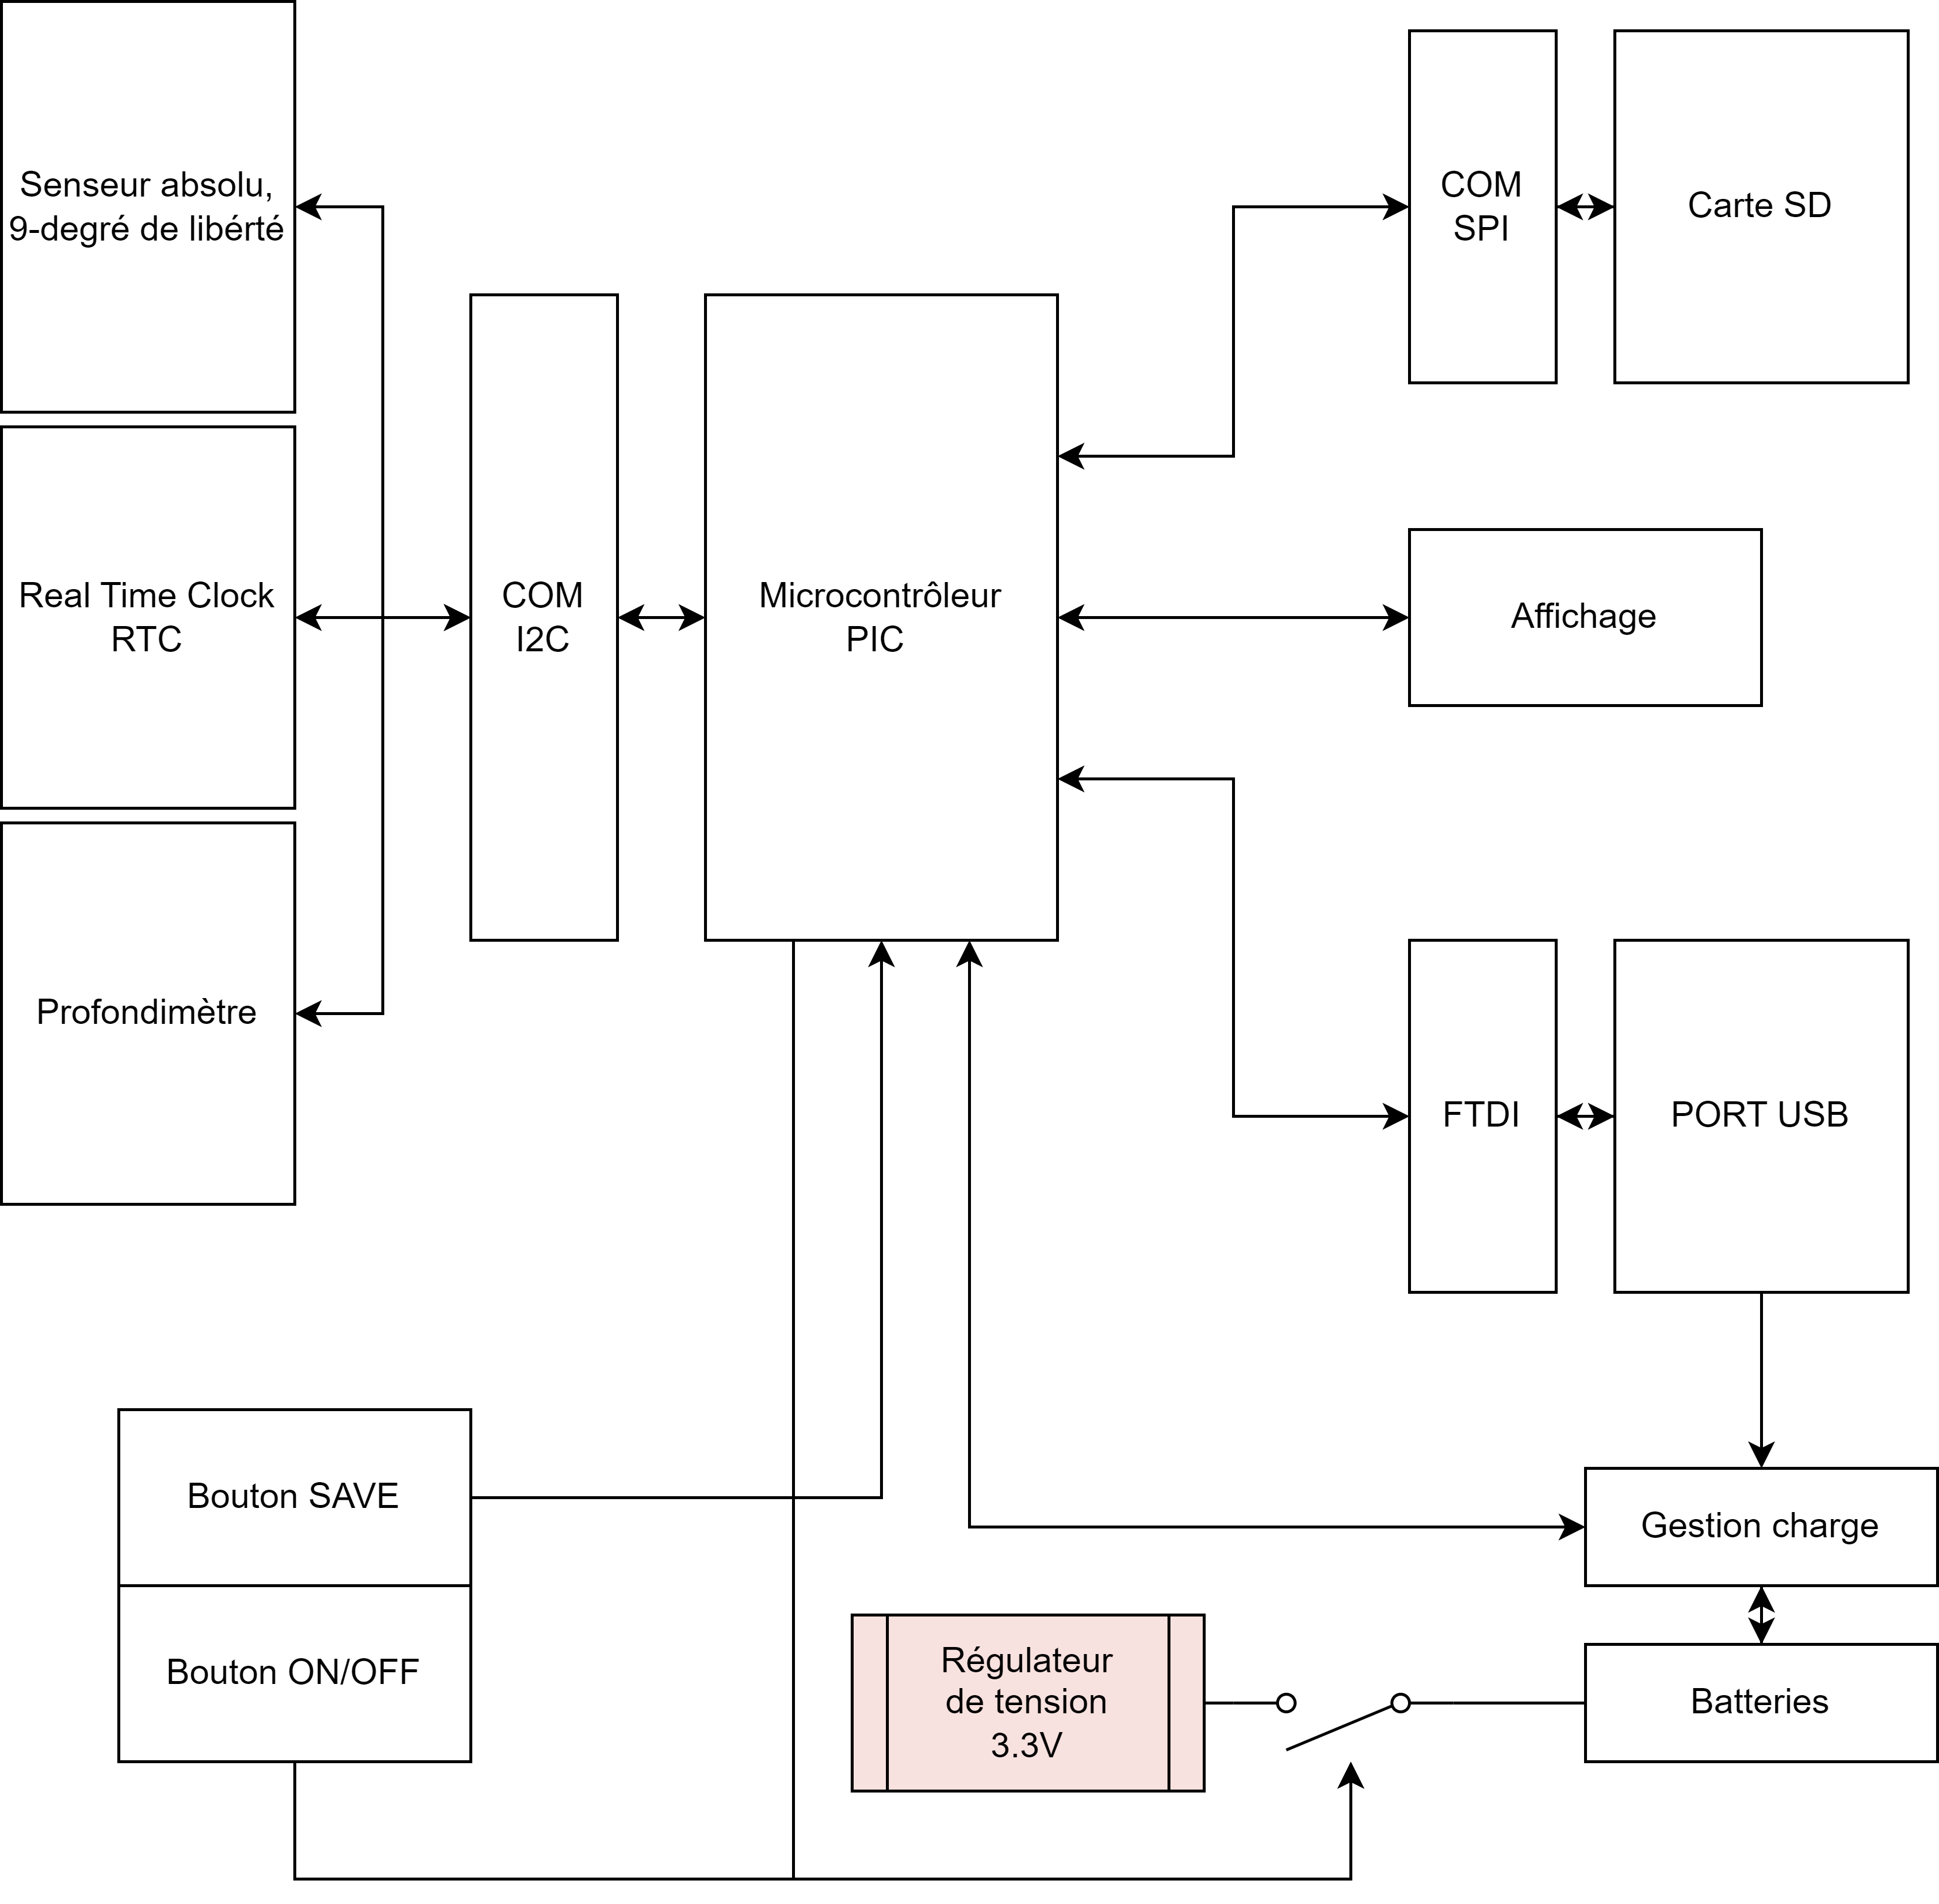
\includegraphics[width=.9\textwidth]{Figures/Schema-bloc-LocalisationSousMarin.drawio}
    \caption{Schéma bloc du module}
    \source{Auteur}
    \label{fig:SchemaBloc}
\end{figure}

\clearpage

\paragraph{Capteurs :} 
Les différents capteurs sont interfacés sur le même bus, et ont comme master le microcontrôleur en communication bidirectionnel, afin d'à la fois configurer les registres des périphériques et de lire leurs mesures.

\paragraph{Carte SD :}
La carte SD est interfacée en SPI et va contenir les données des différents capteurs ainsi que leurs éventuels flags d'importance (sauvegarde), sa taille sera dimensionnée ultérieurement.

\paragraph{Port USB \& charge :}
Un port USB est présent, afin charger les batteries par un IC de gestion de charge connecté directement au 5V. De plus le port USB est communiquant avec le microcontrôleur par un driver FTDI, afin d'éventuellement ajouter un système de lecture de la carte SD, directement par USB. Ceci dans cette version ou une ultérieure. Le port USB pourrait aussi servir a fixer la référence de la RTC. 

\paragraph{Bouton multifonction :}
Sachant qu'un bouton étanche est déjà présent sur le module, l'exploiter en tant que bouton multifonction est une solution ergonomique pour ne pas mettre en péril l'étanchéité globale. Ce bouton ferait office de ON/OFF et de "sauvegarde" de point d'intérêt. Pour se faire, le bouton contrôlerait par un transistor de commutation l'alimentation du système, puis lors de l'allumage du microcontrôleur, le MCU prendrait la relève en maintenant le système allumé a sont tour, permettant ainsi de lire le bouton et de sur une pression longue déconnecter l'alimentation.

\paragraph{Affichage :}
L'affichage permettra de visualiser différentes données, dont les plus importantes tel que la pression ou le statut de la batterie. La forme de l'affichage est encore a définir selon la mécanique du module, mais le plus élégant, serait l'utilisation d'un petit écran OLED.

\paragraph{Capteur de pression :}
Le capteur de pression devra avoir un contact direct avec l'eau, cela impliquera de la mécanique et de la gestion d'étanchéité. Une autre possibilité aurait été de mesurer optiquement la déformation du boîtier pour en déduire la pression, mais la complexité est trop importante.
}

\clearpage

% ----------------Subsection 2 ----------------
\subsection{Choix des composants importants} \label{ssec:num02}
{

\subsubsection{Senseur absolu}
{
    Pour le senseur absolu, il existe des IC permettant directement de faire la fusion des senseurs (\textbf{Accéléromètre, gyroscope, magnétomètre et thermomètre}), ce qui épargne toute une phase de calcul chronophage, en permettant directement de lire les \textbf{quaternion, angles de Euler, vecteurs de rotations, cap de direction etc...} directement sur le composant. Il existe différents IC dont deux ce sont montrés très intéressants, le \textbf{BNO85} et le \textbf{BNO55}, les deux étant PIN-Compatibles, j'ai décidé d'opter pour le \textbf{\underline{BNO055}}\footnote{\href{K:/ES/PROJETS/SLO/2221\_LocalisationSousMarine/doc/composants/9DOF-BNO055}{K:/ES/PROJETS/SLO/2221\_LocalisationSousMarine/doc/composants/9DOF-BNO055}}.
    
    \begin{figure}[h]
    \centering
    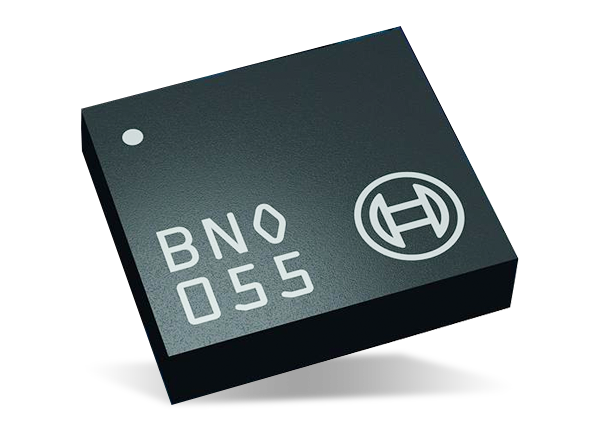
\includegraphics[width=.4\textwidth]{Figures/BNO055-Illustration}
    \caption{Schéma bloc du module}
    \source{\href{https://www.mouser.ch/new/bosch/bosch-bno55-sensor/}{https://www.mouser.ch/new/bosch/bosch-bno55-sensor/}}
    \label{fig:SchemaBloc}
    \end{figure}
    
    Sachant que la brazure de ce type de boîtier est compliquée et également dans un but de simplification du projet, j'ai décidé d'utiliser les cartes d'évaluation d'adafruit \textbf{N°: 4646} qui ont des connections bergs ainsi que tous les composants externes passifs déjà montés. \\
    
    \underline{Caractéristiques importantes :} \\
    
    \begin{tabular}{l l l l}
        Résolution gyroscope & : & 16 & [bits] \\
        Résolution accéléromètre & : & 14 & [bits] \\
        Résolution magnétomètre & : & $\sim$0.3 & [$\mu$T] \\
        $I_{DD}$ & : & 12.3 & [mA] \\
        Dérive de température & : & $\pm$ 0.03 & [\%/K] \\ 
        Dérive accéléromètre & : & 0.2 & [\%/V] \\
        Dérive gyroscope & : & <0.4 & [\%/V]
    \end{tabular} \\
    Nous allons par la suite voir sur la figure \ref{fig:BnoOut}, quelles données du BNO055 sont disponibles ainsi que leurs tailles mémoires.
    
    \begin{figure}[h] 
        \centering
        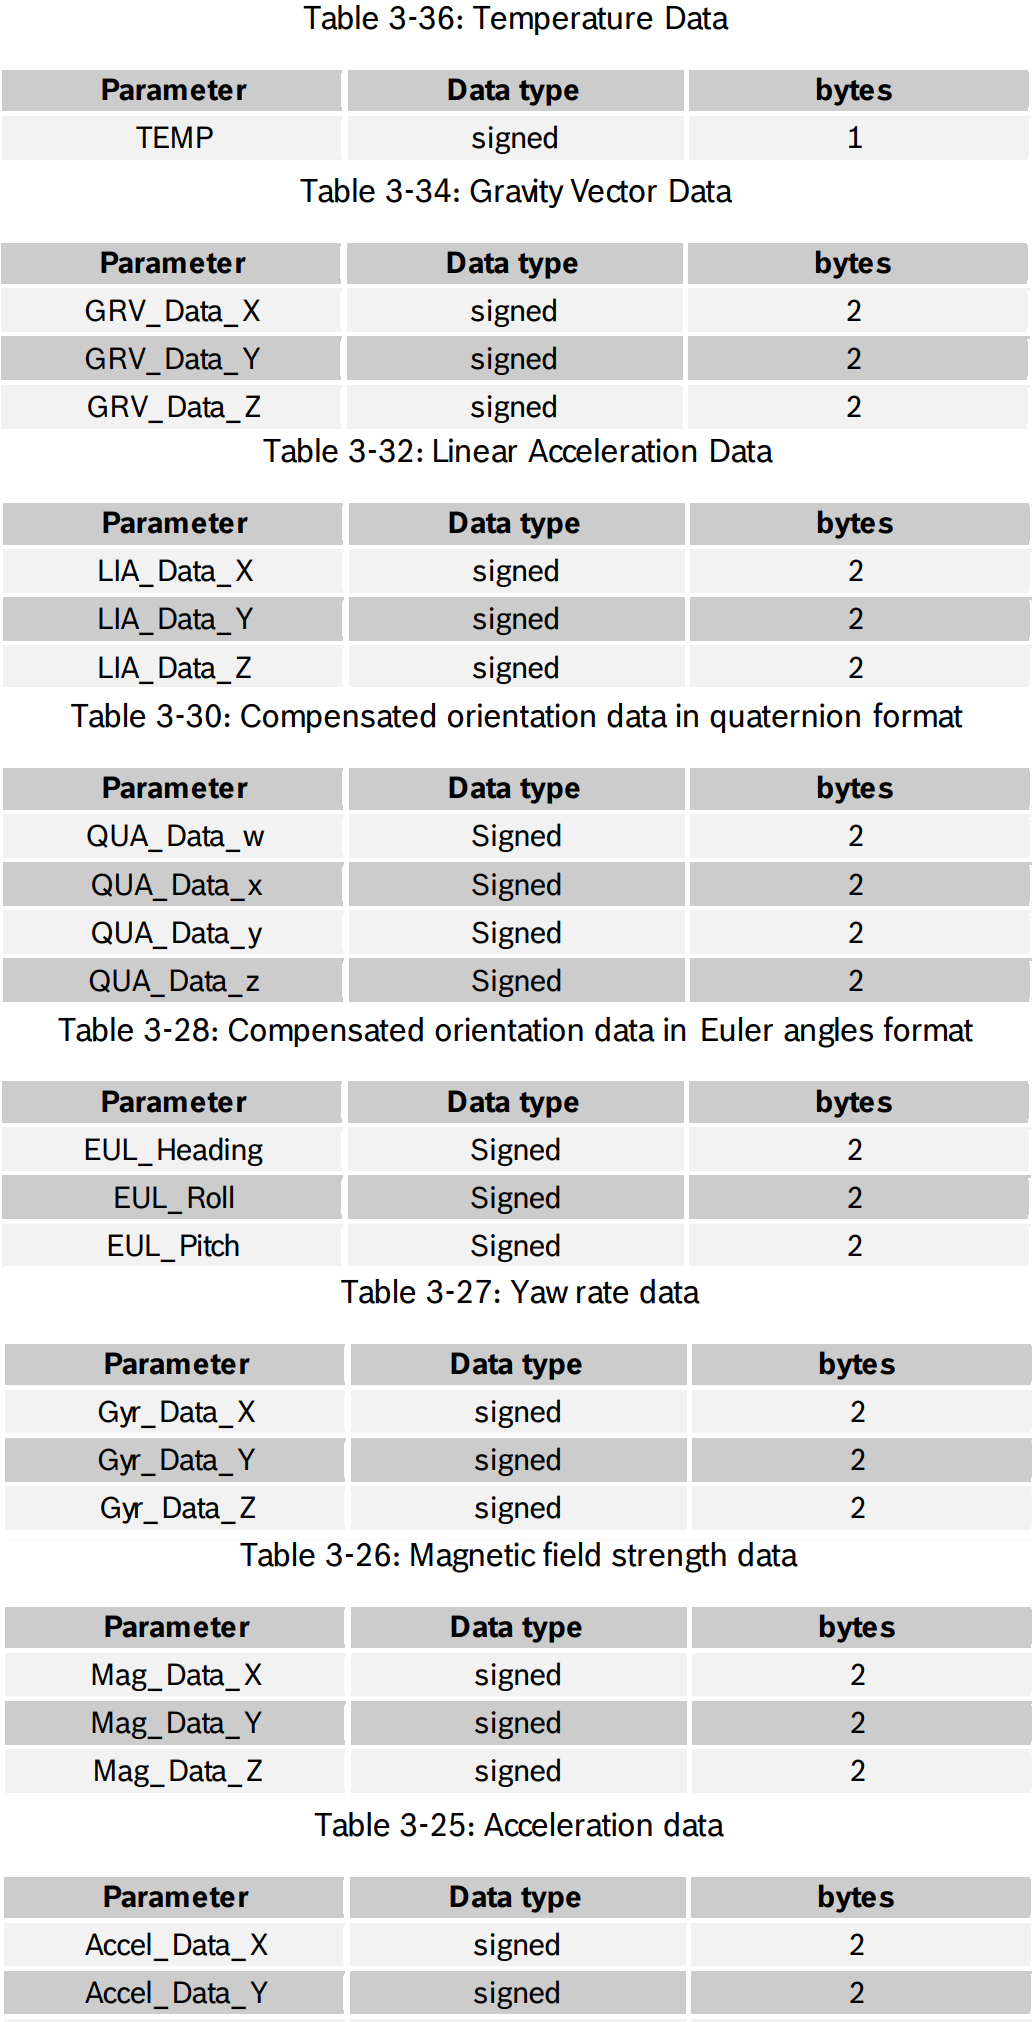
\includegraphics[width=.68\textwidth]{Figures/DATAS-BNO055}
        \caption{Donnée de sortie de l'IC (43 bytes)}
        \source{ \href{https://cdn-shop.adafruit.com/datasheets/BST\_BNO055\_DS000\_12.pdf}{https://cdn-shop.adafruit.com/datasheets/BST\_BNO055\_DS000\_12.pdf} }
        \label{fig:BnoOut}
    \end{figure}
}

\clearpage

\subsubsection{Capteur de pression}
{
Pour le capteur de pression, une modification mécanique du boîter sera très probablement nécessaire. J'ai pu trouver un capteur correspondant aux caractéristiques demandée du projet, celui-ci est plutôt générique et peut communiquer en I2C : \\
\textbf{PTE7300-14AN-1B016BN}

\begin{figure}[h] 
    \centering
    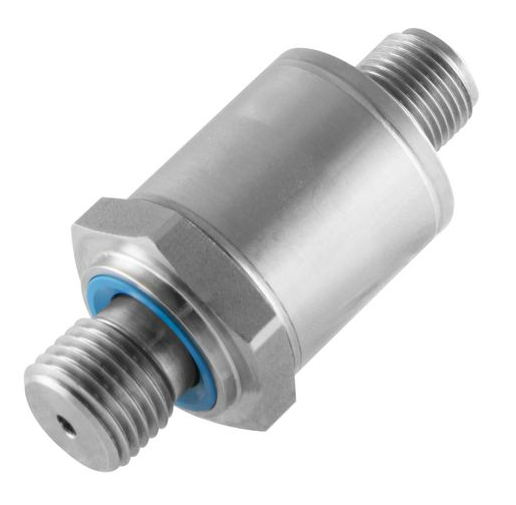
\includegraphics[width=.4\textwidth]{Figures/Capteur-pression}
    \caption{Illustration capteur de pression}
    \source{Distrelec, \href{https://www.distrelec.ch/fr/capteur-de-pression-hermetique-numerique-industriel-g1-16bar-module-sensata-pte7300-14an-1b016bn/p/30302457}{PTE7300-14AN-1B016BN}}
    \label{fig:CaptPress}
\end{figure}

L'avantage avec le capteur ci-dessus est le système hermétique pour le trou, un autre capteur peut être utilisé lors de l'étude, néanmoins la modification mécanique étant probablement inévitable, le système de vissage de la figure \ref{fig:CaptPress} est intéréssant.

}

\subsubsection{Affichage}
{
    Pour l'affichage, je vais essayer d'opter pour un petit afficheur OLED, en gardant la possibilité en cas de de complication lors de l'étude, l'utilisation de simples LEDS d'indications.
    \\
    Il existe plusieurs affichages OLED rond petits formats, sur lesquels je me pencherais plus en détail lors de l'étude.
    


}

\newpage
\subsubsection{Carte SD} \label{sssec:CarteSD}
{
    \paragraph{Taille mémoire : }
    Afin de dimensionner la taille de stockage de la carte SD, il faut utiliser les différentes caractéristiques du projet. Normalement la taille de la carte SD n'est clairement pas un problème, sachant que seulement du texte est enregistré et que les tailles mémoires disponibles peuvent être très élevées. Néanmoins il est intéressant de faire le dimensionnement pour connaître le minimum, et pour éventuellement adapter le projet avec d'autres systèmes de mémorisation.  \\
    Où : \vspace{+14pt} \\
    \begin{tabular}{l l ll|l}
       $ T_{rec} $ & = &  $7200'000$ & $[ms]$ & Temps a enregistrer \\
       $ T_{ech}$ & = & $100$  & $[ms]$ & Temps d'un échantillon \\
       $ S_{mes} $ & = & $150$ & $[bytes]$ & Taille de toutes les données de mesures  \\
       $ S_{timestamp} $ & = & $\sim$3 & $[bytes]$ & Taille de l'information de temporalité  \\
       $ S_{flag} $ & = & $ 1 $ & $[bytes]$ & Taille de l'indication d'importance 
    \end{tabular}
    \vspace{+14pt}
    \\
   \paragraph{ Nombre de mesure a effectuer :}
    \begin{equation} \label{equ:NbMes}
        Nb_{mesures} = \frac{T_{rec}}{T_{ech}}
    \end{equation} 
    D'après (\ref{equ:NbMes}), nous avons un nombre de mesure de 72'000.  \vspace{+8pt} \\
    
   \paragraph{Taille minimum :}
    \begin{equation} \label{equ:TailleMin}
        Taille_{min} = Nb_{mesures} * (S_{mes}+S_{timestamp}+S_{flag}) 
    \end{equation}
    D'après (\ref{equ:TailleMin}), la taille mémoire minimum doit être de \textbf{$\sim$11MB}. \vspace{+8pt} \\ 
    Nous pouvons donc constater que pour une utilisation standard de 2h, la mémoire occupée est très faible, d'où l'intérêt de sauvegarder dans la carte SD la date, afin de pouvoir faire plusieurs "expéditions" en "une fois", sans avoir à vider la carte.
}

\newpage
\subsubsection{Real Time Clock}
{
    L'objectif de la RTC, est de donner l'information de la temporalité de la mesure (timestamp), afin de lors du traitement des donnée avoir accès à ce paramètre. \\
    Sachant que l'échantillonnage des mesures est de 100ms, la RTC devrait permettre cette résolution. Néanmoins une autre information importante, comme mentionnée lors de la section \ref{sssec:CarteSD}, est la date de la mesure, afin de permettre plusieurs expéditions par utilisation de la carte. \vspace{+8pt} \\
    J'ai donc décidé d'utiliser une RTC pour l'heure grossière de départ (Année, date, heure, minute, seconde) et les compteur du MCU pour faire le delta entre chacune des mesures en ms. \\

    La RTC devra pouvoir tenir le minimum de 2 heure d'utilisation, à cette fin, la batterie LI-ION déjà présente sera suffisante. \\ 
    La RTC devra avoir une faible consommation, le calendrier ainsi qu'une bonne précision. A cette fin, la RTC \textbf{S-35390A-T8T1G} est assez générique et possède une bonne documentation.
     
    
}

\subsubsection{Microcontrôleur}
{
    Le microcontrôleur devra avoir un nombre suffisant de communications, sachant que beaucoup sont présentes dans le projet (\textbf{I2C, SPI, UART...}), ce qui signifie un nombre de pattes élevées. 
    
    
    Des calculs peuvent aussi être nécessaire, si il s'avère qu'il faille faire une traitement des données préliminaire, il faudrait donc opter pour un MCU 32bits si possible.


    La famille PIC est celle standardisée par l'école supérieure, c'est donc pour cette famille-ci que je vais opter.
    \vspace{+12pt} \\

    \begin{figure}[h] 
        \centering
        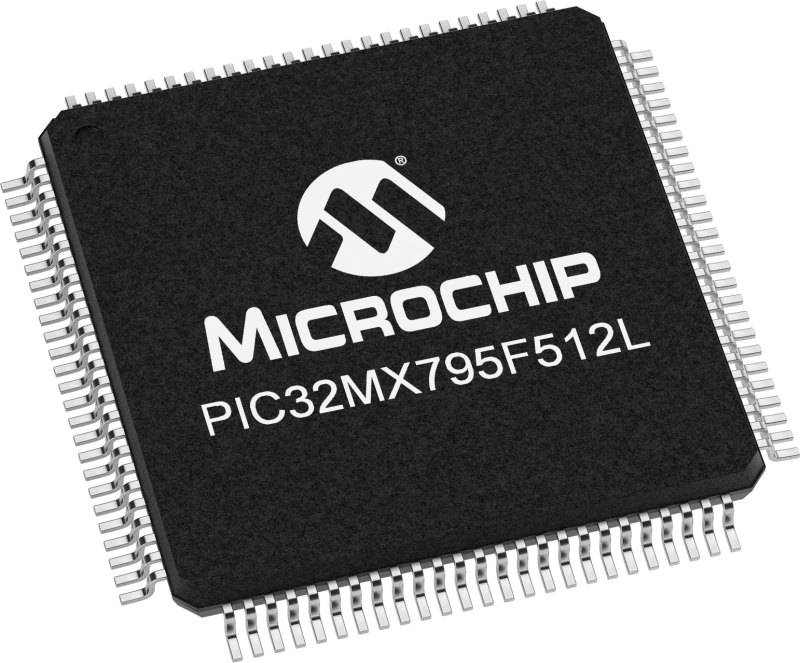
\includegraphics[width=.4\textwidth]{Figures/PIC32MX795F512L-V7X-Regular}
        \caption{Illustration du modèle MCU du kit ETML-ES}
        \source{\href{https://www.microchip.com/en-us/product/PIC32MX795F512L}{https://www.microchip.com/en-us/product/PIC32MX795F512L}}
        \label{fig:MCU}
    \end{figure}
    
}

\clearpage

\subsubsection{Batterie, charge et régulation}
{

Pour la technologie de batterie, en utilisation sous-marine, j'ai trouvé ce tableau de comparaison :

\begin{figure}[h]
    \centering
    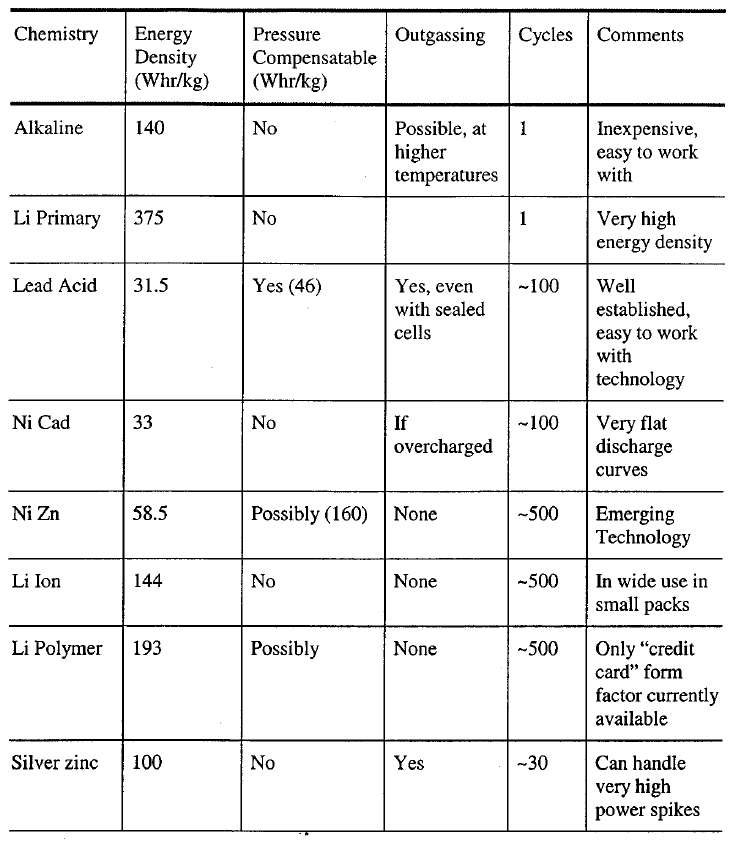
\includegraphics[width=.56\textwidth]{Figures/PowerSystemsComparison}
    \caption{Comparaison des technologies de batteries}
    \source{Power Systems for Autonomous Underwater Vehicles\cite{bradley_power_2001}}
    \label{fig:BatteriesComparaisons}
\end{figure}

Pour des raisons de praticité et étant-donné la documentation plus importante, j'ai décidé d'utiliser la technologie \textbf{LI-ION} : \\

\begin{table}[h]
	\centering
	\begin{tabular}{l|l}
		Avantages &  Inconvénient\\
		\hline
		Haute densité d'énergie & Risque d'éclatement \\
		Poids léger & Risque d'enflammement avec l'eau \\ 
		Haute durée de vie & Sensible a la température \\
		Charge rapide & Décharge complète altérante \\
	\end{tabular}
	\caption{Tableau avantages/inconvénient LI-ION)}
\end{table}

\vspace{+8pt}

Malgré les risque dûs au contact de l'eau (\textbf{Enflammement, éclatement...}) la technologie LI-ION est souvent utilisée pour les application sous-marines dû a ses différents avantages, c'est pour cela que j'opterais pour cette technologie. 

}

}

\newpage
\subsection{Estimation des coûts} \label{ssec:EstPrix}
{
    Ici je vais me baser sur les composants que j'ai pu trouver et estimer le coût moyen de ceux-ci, c'est a titre purement indicatif, (les prix sont généralement estimés a la hausse).
    \vspace{+12pt}
    
    \begin{center}
        \begin{tabular}{l|l}
            Composant & Estimation \\
            \hline
            Profondimètre & 70.- \\
            Centrale inertielle & 35.- \\
            RTC & 5.- \\
            Microcontrôleur & 5.- \\
            Carte SD & 20.- \\
            Affichage OLED & 45.- \\
            FTDI & 4.- \\
            Batterie LI-ION & 20.- \\
            IC chargeur & 4.- \\
            Traco-power 3.3V & 10.- \\
            PCB & 40.- \\
            \hline
            \hline
            Total & 258.-
        \end{tabular} 
    \end{center}
	

    L'estimation des prix étant plutôt élevée, des économies peuvent être très facilement réalisées, en changeant l'affichage OLED pour des LEDS ou en modifiant le PCB (Le simplifier ou changer de fournisseur (eurocircuit)).

}

\subsection{Synthèse développement} \label{ssec:PreeConc}
{

J'ai pu lors de cette pré-étude, établir le fonctionnement global du système, choisir certaines technologies et composants importants, ainsi que pu procéder a certains dimensionnements utiles quant au futur développement. 
Par la suite, je vais affiner les différents éléments abordés lors de la pré-étude, effectuer le développement plus détaillé de chacun des blocs et réaliser la schématique du projet.
Lors de la pré-étude, je n'ai pas eu accès au boîtier mécanique du projet, ce qui a restreint mon champs d'action lors de certains dimensionnement, tandis que pendant l'étude j'aurais accès a celui-ci, ce qui risque d'impacter/modifier certains aspect fixés lors des section antérieures.
Je suis très intéressé par le projet et me réjouis grandement de poursuivre son développement.

}

\clearpage
